\section{ХОД РАБОТЫ}

\subsection{Текст задания}

Данная лабораторная работа выполняется на основе предыдущих лабораторных работ №4-6.

На рисунке~\ref{lst:task_struct} представлена структура, содержащая массив элементов типа Complex.

\begin{lstlisting}[caption=Структура\text{,} содержащая массив элементов типа Complex,label=lst:task_struct]
  #define COMPLEXES_SIZE 5

  struct Complexes {
    int count;
    int complexes_size;
    struct Complex complexes[COMPLEXES_SIZE];
  };
\end{lstlisting}

Главный поток программы (функция main()) создаёт вторичный поток, передав в него указатель на структуру типа Complex. Вторичный поток запоминает значение из поля count, открывает файл, и затем в цикле, если значение count изменилось, записывает элементы массива complexes в файл. После этого поток закрывает файл и завершается.

Главный поток организует цикл ввода комплексных чисел следующим образом:

\begin{itemize}
  \item инициализируется временная переменная типа Complex (ввод числа с клавиатуры);
  \item c помощью функции SuspendThread() приостанавливается поток;
  \item значение переменной заносится в массив типа Complex;
  \item с помощью функции ResumeThread() поток запускается на выполнение.
\end{itemize}

\newpage

\subsection{Исходные данные}


На рисунках~\ref{lst:complex_h_code}~-~\ref{lst:file_io_h_code} представлено содержимое наиболее важных заголовочных файлов, реализованных в предыдущих лабораторных работах.

\begin{lstlisting}[caption=Исходный код заколовочного файла complex.h,label=lst:complex_h_code]
  #ifndef __COMPLEX__
  #define __COMPLEX__

  struct Complex {
      double re;
      double im;
  };
  struct Complex add(struct Complex c1, struct Complex c2);
  struct Complex sub(struct Complex c1, struct Complex c2);
  struct Complex mul(struct Complex c1, struct Complex c2);
  struct Complex division(struct Complex c1, struct Complex c2, int * error);

  void writeComplex(char *fname, struct Complex *complex, int count);
  int readComplex(char *fname, struct Complex *complex, int count);

  #endif
\end{lstlisting}

\begin{lstlisting}[caption=Исходный код заколовочного файла complex\_io.h,label=lst:complex_io_h_code]
  #ifndef __COMPLEX_IO__
  #define __COMPLEX_IO__

  struct Complex input_complex();
  void print_algebraic_form(struct Complex complex);
  void print_polar_form(struct Complex c);
  void print_complex(struct Complex complex);
  void print_complex_array(struct Complex *complex, int count);

  #endif
\end{lstlisting}

\begin{lstlisting}[caption=Исходный код заколовочного файла file\_io.h,label=lst:file_io_h_code]
  #ifndef __FILE_IO__
  #define __FILE_IO__

  void writeComplex(char *fname, struct Complex *complex, int count);
  int readComplex(char *fname, struct Complex *complex, int count);

  #endif
\end{lstlisting}

Функции, объявленные в изображенных выше заголовочных файлах использовались при выполнении лабораторной работы №7.

\subsection{Особенности разработанной программы}

В ходе проведения данной лабораторной работы была разработана программа для записи комплексных чисел в файл во вторичном потоке.

На рисунке~\ref{fig:uml} проиллюстрировано взаимодействие файлов проекта с помощью диаграммы пакетов UML.

\begin{figure}[htbp]
  \centering
  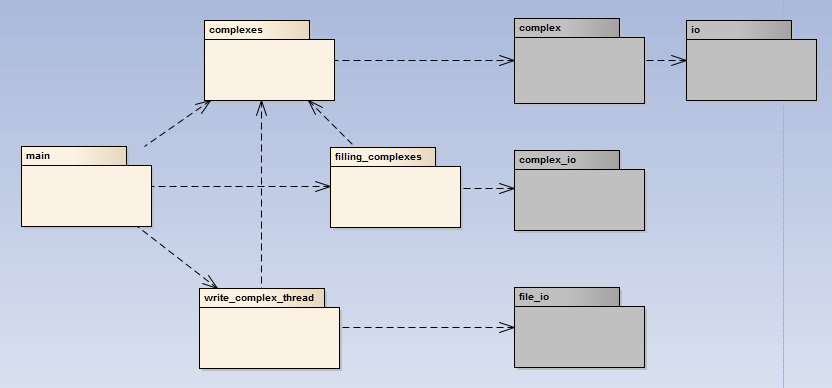
\includegraphics[width=150mm,height=80mm]{img/uml}
  \caption{Диаграмма пакетов UML лабораторной работы №7}\label{fig:uml}
\end{figure}

После запуска программы на выполнение главный поток (функция создаёт вторичный поток, передав в него указатель на функцию записи комплексных чисел в файл. В главном потоке пользователь вводит комплексные числа.

Далее организуется следующий цикл: вторичный поток приостанавливается. Пользователь вводит несколько файлов, затем вторичный поток запускается и происходит запись в файл.

Исходный текст разработанной программы расположен в приложении~А.

\newpage
